%-*- coding:UTF-8 -*-
% 算法导论-第13章 红黑树.tex
\documentclass[UTF8]{ctexart}
\usepackage{geometry}
\usepackage{enumerate}
\usepackage{amsmath}
\usepackage{listings} %插入代码
\usepackage{xcolor} %代码高亮
\usepackage{diagbox}
\usepackage{tabularx}
\usepackage{graphicx}
\usepackage{caption}
\usepackage{subcaption}
\usepackage{float}

% Some setup
\pagestyle{plain}
\geometry{a4paper, top=2cm, bottom=2cm, left=2cm, right=2cm}
\CTEXsetup[format={\raggedright\bfseries\Large}]{section}
\lstset{numbers=left, %设置行号位置
        numberstyle=\small, %设置行号大小
        keywordstyle=\color{blue}, %设置关键字颜色
        commentstyle=\color{purple}, %设置注释颜色
        %frame=single, %设置边框格式
        escapeinside=``, %逃逸字符(1左面的键),用于显示中文
        breaklines, %自动折行
        extendedchars=false, %解决代码跨页时,章节标题,页眉等汉字不显示的问题
        %xleftmargin=2em,xrightmargin=2em, aboveskip=1em, %设置边距
        tabsize=4, %设置tab空格数
        showspaces=false %不显示空格
       }

% About math
\newcommand{\rmnum}[1]{\romannumeral #1}

\begin{document}

\title{\Huge算法导论习题\\}
\vspace{2cm}
\author{\Large曾宇祥\\SY1406122}
\date{}
\maketitle

%\newpage
\section*{第13章\quad红黑树}
\begin{enumerate}
    \item 13.1-2 \\
    解:\\
        均不是,若结点为红色不满足性质4;若结点为黑色不满足性质5.
		
	\item 13.1-3 \\
	解:\\
		仍旧是红黑树,满足性质1-5。
		
	\item 13.1-4 \\
	解:\\
		这个题目描述的不清楚,其实就是把红色结点和黑结点归并到一起组成一个新的结点。因此,\\
		当黑色父结点的子结点均为黑色时,度为2;	\\
		当黑色父结点仅含一个黑色子结点时,度为3;	\\
		当黑色父结点的两个子结点均为红色时,度为4.	\\
		由于红色结点全部被吸收,即仅余下黑结点。由红黑树性质5可知叶结点深度均相同。
	
	\item 13.1-5 \\
	解:\\
		可以先形式化验证, 考虑结点x的黑高为BH(x), 红高为RH(x), 而RH(x)<=BH(x).
		结点x到后代叶结点的最长路径为BH(x)+RH(x), 最短路径为BH(x). 因此,至多为2倍。\\
		再形象地考虑一下路径会是什么样的。\\
		设x的黑高为h,
		当x的颜色为黑色,则最长路径的着色为黑-红-黑-$\cdots$-红-黑-红-黑, 长度为(2h-2),
		最短路径的着色为黑-黑-$\cdots$-黑-黑,长度为(h-1), 比值为2。\\
		当x的颜色为红色,则最长路径的着色为红-黑-红-黑-$\cdots$-红-黑-红-黑, 长度为(2h-1),
		最短路径的着色为红-黑-黑-$\cdots$-黑-黑,长度为h, 比值趋近于2。\\
		因此,综上可知比值最多为2.
		
	\item 13.1-6 \\
	解:\\
		内部结点最多为$2^(2k)-1$, 显然为一棵完全数,每层结点颜色为黑-红交替。\\
		内部结点最少为$2^k-1$,显然为一棵全黑树。
		
	\item 13.1-7 \\
	解:\\
		比值最大为2:1, 比值最小为0(全黑树)。
		
	\item 13.2-2 \\
	证明:\\
		因为红黑树本身就没什么引理或者公理,因此想到使用数学归纳法证明。
		当n=1时,结论显然成立,因为无论左旋还是右旋,根本不会改变二叉搜索树。
		当n=k时,不妨假设当n<k时,恰有n-1种可能的旋转。仅需证明当n=k时,结论同样成立。\\
		从n个结点的二叉搜索树种任取一个叶子结点x,余下n-1个结点,存在n-2种可能的旋转 。
		这意味着x的父节点必将取便n-1个结点,否则对于n-1个结点,至少还有一种旋转。\\
		因此n个结点的旋转总数就是结点x与其父节点旋转后的可能总数(左旋还是右旋取决于两者大小),
		且这n-1种旋转互不相同,即为n-1。\\
		故结论成立。
		
	\item 13.2-3 \\
	解:\\
		a加1,b不变,c减1
		
	\item 13.2-4 \\
	证明:\\
		提示已经很显然。假设二叉搜索树$T_1$与$T_2$包含相同元素(个数相同,值相同)。$|T1| = n$,
		使用n-1次旋转策略$s_1$可以将$T_1$旋转成一条右侧伸展的链,同理$T_2$也可以通过若干次旋转策略$s_2$形成一条右侧伸展的链。\\
		由二叉搜索树的性质可以这两条链完全相同。因此,通过对链$T_0$逆向使用$s_2$即可以形成链$T_2$。\\
		因此,$T(n) < 2n = O(n)$.
		
	\item 13.2-5 \\
	证明:\\
		待研究。
		
	\item 13.3-1 \\
	解:\\
		若将结点z着为黑色,则红黑树的黑高不平衡。破坏性质5,而且难以维护。
		
	\item 13.3-2 \\
	解:\\
		\begin{figure}[H]
		\centering
        \caption{插入41,38,31,12,19,8的红黑树示意图}
		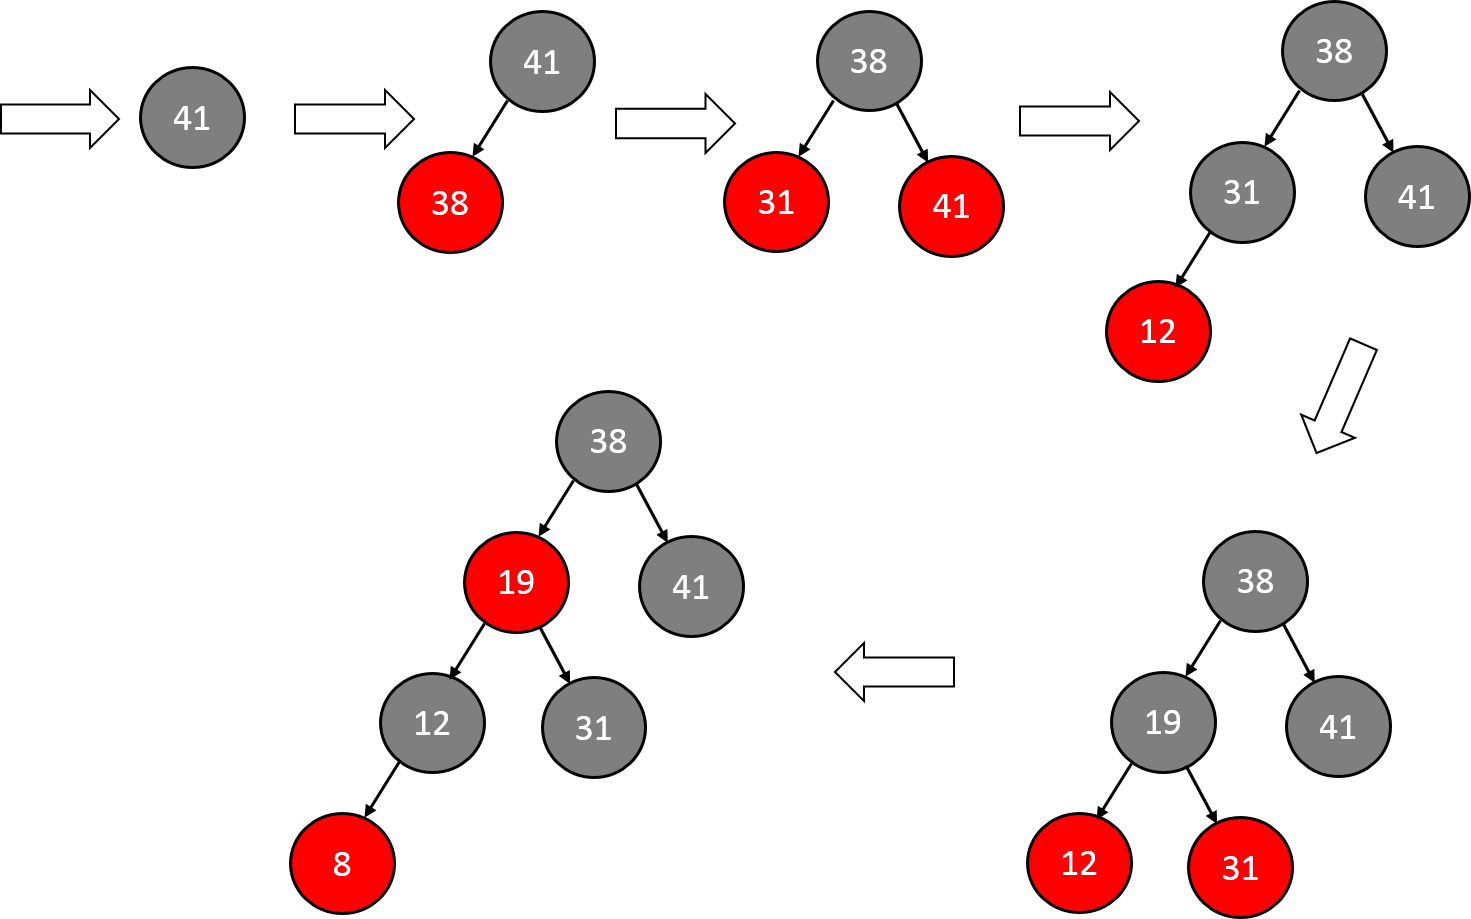
\includegraphics[scale=0.65]{13_3_2.png}
		\end{figure}
		
	\item 13.3-4 \\
	证明:\\
		仅需要证明RB-INSERT-FIXUP过程不会修改T.NIL的color属性即可。首先,需要明确一件事情,
		RB-INSERT-FIXUP是严格维护黑高的(即红黑树性质5),为什么说严格维护黑高?
		相对于RB-DELETE-FIXUP而言。\\
		考虑z为z.p的左子树的情况,z为右子树的情况同理可证。
		程序中仅7行、13行把颜色属性修改为红色。使用反证法证明,假设T.NIL被7行或13行修改为红色。\\
		也即z.p.p==T.NIL, z.p==ROOT。而进行循环的条件为z.p.color==RED,因此当z为根结点的子结点时,
		根本不会进入循环。因此假设错误,易知T.NIL.color恒保持为Black。
	
	\item 13.3-5 \\
	证明:\\
		很显然,其实根本不用数学归纳,算法就是这么做的。RB-INSERT过程将新加入的结点z置为红色,
		当n>1时,原树至少包含根结点。\\
		若z.p.color==BLACK,则不进入RB-INSERT-FIXUP的循环,因此z保持红色不变,此时结论成立。\\
		若z.p.color==RED, 而RB-INSERT过程中并没有改变z的颜色,因此,仍然至少包含一个结点为红色。
	
	\item 13.4-1 \\
	证明:\\
		当x==T.root跳出循环时,x.color=BLACK可以将根结点颜色置为黑色。\\
		当x!=T.root进入循环时,\\
		情况2仅对x的兄弟结点w进行着色(根结点无兄弟结点),因此,显然不会修改根结点的颜色。\\
		情况4若17行将父结点的颜色传递给w,同事对父结点进行左旋,左旋后w成为新的父结点,而w的颜色并没有发生变化。\\
		综上可知,T.root.color恒为黑色。
	
	\item 13.4-2 \\
	证明:\\
		x.color为RED,而原来y的父结点为RED。直接将x的颜色改为BLACK,但这只是最简单的一种情况。
	
	\item 13.4-3 \\
	解:\\
		\begin{figure}[H]
		\centering
        \caption{删除8,12,19,31,38,41的红黑树示意图}
		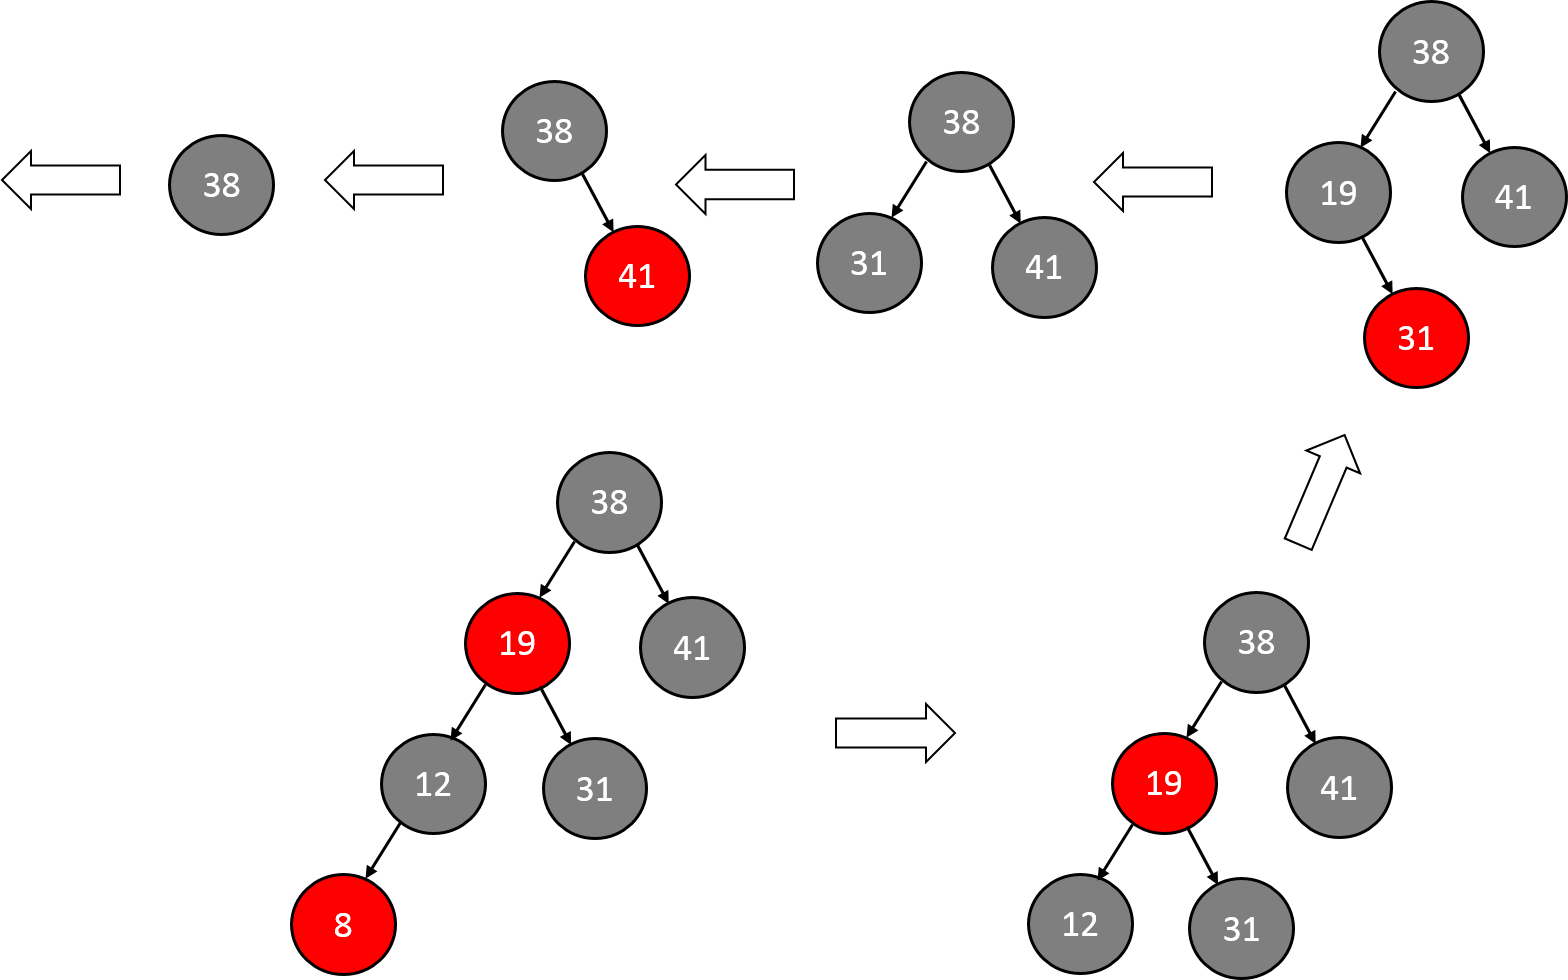
\includegraphics[scale=0.65]{13_4_3.png}
		\end{figure}
	
	\item 13.4-6 \\	
	证明:\\
		情况1开始时,w.color==RED, 因此w.p.color=BLACK(红黑树性质),而w.p==x.p,因此当情况1发生时,x.p.color==BLACK恒成立。
		
	\item 13.4-7 \\
	证明:\\
		不一定一样,着色可能会不一样。可以写个随机数发生器实际测试一下。
	
\end{enumerate}


\end{document}

